% !TEX root = ../report.tex

\clearpage
\chapter{Evaluation}
\label{ch:evaluation}
This chapter presents the evaluation of documented patterns and overall system
against the key drivers of the architecture which already presented in Chapter
\ref{ch:stakeholders}. PBAR\cite{pbar} method is used to carry out the
evaluation. Force Resolution Maps (FRM) are also utilized to present the result.

\begin{table}[H]
\centering
\caption{Force Resolution Maps definition.}
\label{tab:frm-table}
\begin{tabular}{cl}
\textbf{Value} & \textbf{Definition} \\ \toprule
            $-2$   & Big negative impact \\
            $-1$   & Small negative impact \\
            $0$    & Neutral \\
            $+1$   & Small positive impact \\
            $+2$   & High positive impact 
\end{tabular}
\end{table}

\section{Patterns}
%TODO: some text must be here

\subsection{Client-Server}
\begin{figure}[H]
\centering
\includegraphics[scale=0.7]{6-evaluation/images/clientserver_frm.png}
\caption{Force Resolution Map for Client-Server pattern}
\label{fig:clientserver-frm}
\end{figure}
For the Client-Server pattern, the portability of the system increases, because the client and server (daemon) can be located on completely different systems.

The security has a slight negative impact because for communication between the client and server to be possible, the client and server have to expose an interface, which has to be secured. 

Reliability also has a small negative impact, because the communication between client and server relies on underlying communication infrastructure that could fail. 

\subsection{Layers}

\begin{figure}[H]
\centering
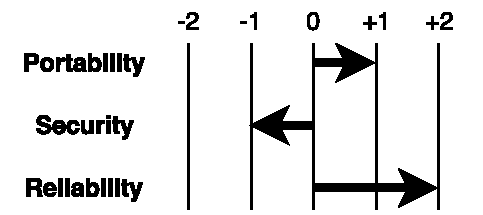
\includegraphics[scale=0.7]{6-evaluation/images/layers_frm.pdf}
\caption{Force Resolution Map for Layers pattern.}
\label{fig:layers-frm}
\end{figure}
This pattern gives positive implication to portability as clear separation of
containers, Docker daemon, Docker registry, and Docker client makes Docker
portable and loosely coupled. Utilizing Docker registry also promotes sharing
images, which make it easier to deploy an application without knowing what
platform running below it. Exposing TCP/IP connection, specifically REST,
contributes to negative effect on the security. It means that any unwanted
connections or attacks could possible exploit this hole. However, this weak
point is compensated by other patterns. 

Furthermore, decoupling some components
means that the components below or above can be replicated in order to gain more
reliability as it has more availability. Thus, this patterns give positive
effect to the reliability. 

The summary of the Layers pattern evaluation is shown
in FRM in Figure \ref{fig:layers-frm}.

\subsection{Plugin}
\begin{figure}[H]
\centering
\includegraphics[scale=0.7]{6-evaluation/images/plugin_frm.png}
\caption{Force Resolution Map for Plugin pattern}
\label{fig:plugin-frm}
\end{figure}
The Plugin pattern greatly increases the portability, because it increases the adaptability by allowing third parties to develop extensions for Docker. 

It has a slight negative impact on the security, because there is communication between the daemon and plugin process which has to be secured. Additionally, the security of the plugins is not controlled by Docker, so defects in a plugins security can affect the security of the Docker daemon as well. 

There are no significant impacts on the reliability because of this pattern.

\subsection{Broker}
\begin{figure}[H]
\centering
\includegraphics[scale=0.7]{6-evaluation/images/broker_frm.png}
\caption{Force Resolution Map for Broker pattern}
\label{fig:broker-frm}
\end{figure}
The use of the Broker pattern is very beneficial for the portability, because it allows the use of components in different processes, potentially running on different machines.

This pattern is also positive for the security of Docker, because it is a single entrypoint for all inter-process communication, which is easier to secure than multiple entrypoints.

%TODO: reliability

\subsection{Proxy}
\begin{figure}[H]
\centering
\includegraphics[scale=0.7]{6-evaluation/images/proxy_frm.png}
\caption{Force Resolution Map for Proxy pattern}
\label{fig:proxy-frm}
\end{figure}
The use of the Proxy pattern has a positive impact on the portability, because the location of the component accessed through the proxy is transparent for the caller.
There is a small negative impact on security, because the invocation on the Proxy are forwarded to the component in another process. This communication has to be secured.


\subsection{Shared/Active repository} 
The use of the Shared Repository patterns has different impacts on the differents Key Drivers : 
% Explaining how it works and the KD matched
Reliability \\
Security is enhanced because the repository is central so has its access who is controlled by a login for the users. \\
Portability \\

\subsection{Publish Suscribe}

The publish subscribe pattern allows the event occuring in the Docker Registry to be triggered to the user who has previously subscribed to them. When those events happen the user receives a webhook notification.
% Mechanism :
% Endpoint, Http

Reliability \\
Security \\
Portability \\

\subsection{Brokered Authentication}
% Process 
Reliability \\
Security \\
Portability \\


\section{Overall system}